\documentclass[aspectratio=169]{beamer}

\usepackage[utf8]{inputenc}
\usepackage[T1]{fontenc}
\usepackage[english]{babel}
\usepackage{graphicx}
\usepackage{amsmath,amssymb}
\usepackage{tikz}
\usetikzlibrary{positioning,arrows.meta,shapes.geometric}

% --- PWr color scheme (same as ICAISC 2026 / SOCO templates) ---
\xdefinecolor{pwrone}{rgb}{0.6015625,0.203125,0.17578125}
\xdefinecolor{pwrtwo}{rgb}{0.94140625,0.81640625,0.6328125}
\definecolor{cadj}{HTML}{5B7DB1}
\definecolor{cfib}{HTML}{9A342D}
\definecolor{cdyn}{HTML}{E08A1E}
\definecolor{cmot}{HTML}{2A9D8F}
\mode<presentation>
{
    \usetheme{Warsaw}
    \setbeamercolor{structure}{fg=pwrone}
    \setbeamercolor*{palette primary}{use=structure,fg=pwrtwo,bg=pwrone}
    \setbeamercolor*{palette quaternary}{use=structure,fg=pwrone,bg=pwrtwo}
}
\usetheme{Warsaw}
\setbeamertemplate{navigation symbols}{}

% --- Frame counter in footer ---
\newcommand*\oldmacro{}
\let\oldmacro\insertshortauthor
\renewcommand*\insertshortauthor{%
    \leftskip=.3cm%
    \insertframenumber\,/\,\inserttotalframenumber\hfill\oldmacro%
}

\newcommand{\nbarc}[4]{\pgfmathsetmacro\xa{((#2+.5)*\linewidth/4+(#3-3)*.42cm)/1cm}\pgfmathsetmacro\xb{((#2+.5)*\linewidth/4+(#4-3)*.42cm)/1cm}\draw[very thick,#1] (\xa,0) to[bend left=75] (\xb,0);}
\newcommand{\takeaway}[1]{\par\vspace{2mm}\centering\colorbox{pwrtwo}{\parbox{.92\linewidth}{\centering\strut #1\strut}}}

\title[Gate-Model Quantum Neighborhood Search for the PFSP]
{Gate-Model Quantum Neighborhood Search\\
for the Permutation Flow Shop Problem\\
via Fixed-Angle QAOA}
\author[R.~Wojew\'odzki, W.~Bo\.zejko]
{Remigiusz Wojew\'odzki \and Wojciech Bo\.zejko}
\institute{
Department of Control and Quantum Computing\\
Wroc\l{}aw University of Science and Technology\\[1mm]
{\tt remigiusz.wojewodzki@pwr.edu.pl}\quad\raisebox{-3mm}{
\includegraphics[height=8mm]{logo_PWR.png}}
}
\date{GCMM 2026, Wroc\l{}aw}

\begin{document}

% ===== 1. TITLE =====
\frame{\thispagestyle{empty}\titlepage}

% ===== 2. IDEA =====
\section{Idea}
\begin{frame}{One QUBO, two quantum back-ends}
    \centering
    \begin{tikzpicture}[scale=.85,transform shape,
        box/.style={draw,rounded corners,align=center,minimum height=1.25cm,thick},
        >={Stealth[length=3mm]}]
        \node[box,fill=pwrtwo,minimum width=2.8cm] (ls) at (0,0) {\textbf{ILS / SA}\\\small current $\pi$};
        \node[box,fill=pwrone!25,minimum width=3.2cm] (q) at (4.3,0) {\textbf{neighborhood}\\\textbf{as QUBO}\\\small $\min \mathbf{x}^{\mathsf T}Q\mathbf{x}$};
        \node[box,fill=gray!15,minimum width=3.4cm] (a) at (9.2,1.1) {quantum annealer\\\small earlier work};
        \node[box,fill=pwrone,text=white,minimum width=3.4cm] (g) at (9.2,-1.1) {\textbf{gate-model QAOA}\\\small this talk};
        \draw[->,thick] (ls) -- (q);
        \draw[->,thick] (q.east) -- (a.west);
        \draw[->,thick] (q.east) -- (g.west);
        \draw[->,thick,dashed] (a.east) -- ++(.6,0) |- (5.5,2.5) -| (ls.north) node[pos=.25,above]{\small move = set of disjoint swaps};
        \draw[->,thick,dashed] (g.east) -- ++(.6,0) |- (5.5,-2.5) -| (ls.south);
    \end{tikzpicture}
    \takeaway{Same matrix $Q$, same ILS/SA, same instances --- only the solver changes.}
\end{frame}

% ===== 3. NEIGHBORHOODS =====
\section{Method}
\begin{frame}{Four neighborhoods $\to$ four conflict graphs}
    \centering
    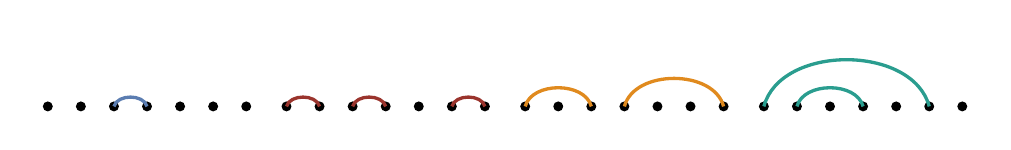
\begin{tikzpicture}
        \useasboundingbox (0,-.2) rectangle (\linewidth,1);
        \foreach \k in {0,...,3} \foreach \i in {0,...,6} {\pgfmathsetmacro\xp{((\k+.5)*\linewidth/4+(\i-3)*.42cm)/1cm}\fill (\xp,0) circle (1.8pt);}
        \nbarc{cadj}{0}{2}{3}
        \nbarc{cfib}{1}{0}{1}\nbarc{cfib}{1}{2}{3}\nbarc{cfib}{1}{5}{6}
        \nbarc{cdyn}{2}{0}{2}\nbarc{cdyn}{2}{3}{6}
        \nbarc{cmot}{3}{0}{5}\nbarc{cmot}{3}{1}{3}
    \end{tikzpicture}\\[1mm]
    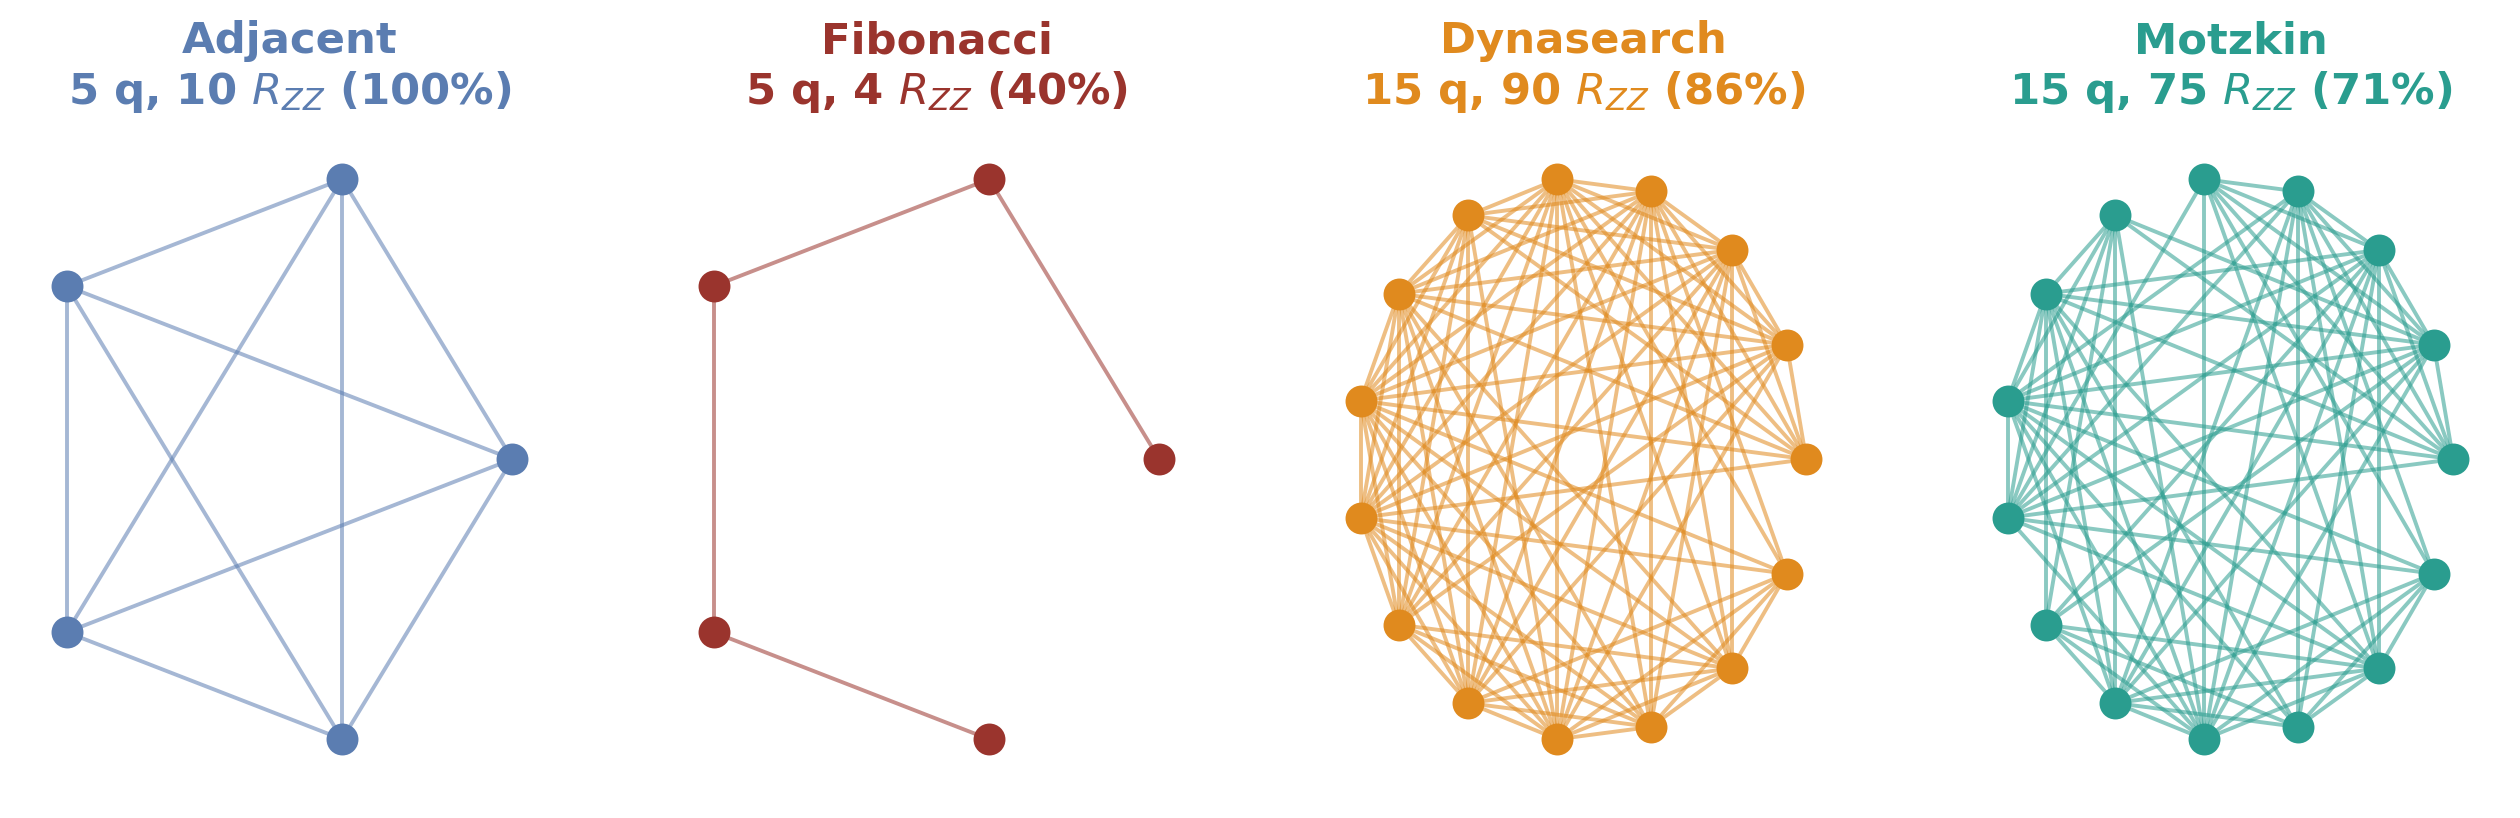
\includegraphics[width=\linewidth,height=.5\textheight,keepaspectratio]{img/conflict_graphs.png}
    \takeaway{One qubit per swap candidate, one $R_{ZZ}$ gate per conflict (6-job window shown).}
\end{frame}

% ===== 4. CIRCUIT =====
\begin{frame}{From QUBO to a $p=1$ QAOA circuit}
    \centering
    $x_k=\tfrac{1+Z_k}{2}\;\Rightarrow\; H_C=\sum_i h_i Z_i+\sum_{i<j}J_{ij}Z_iZ_j$
    \qquad
    $\lvert\gamma,\beta\rangle = e^{-i\beta H_M}e^{-i\gamma H_C}\lvert+\rangle^{\otimes K}$\\[3mm]
    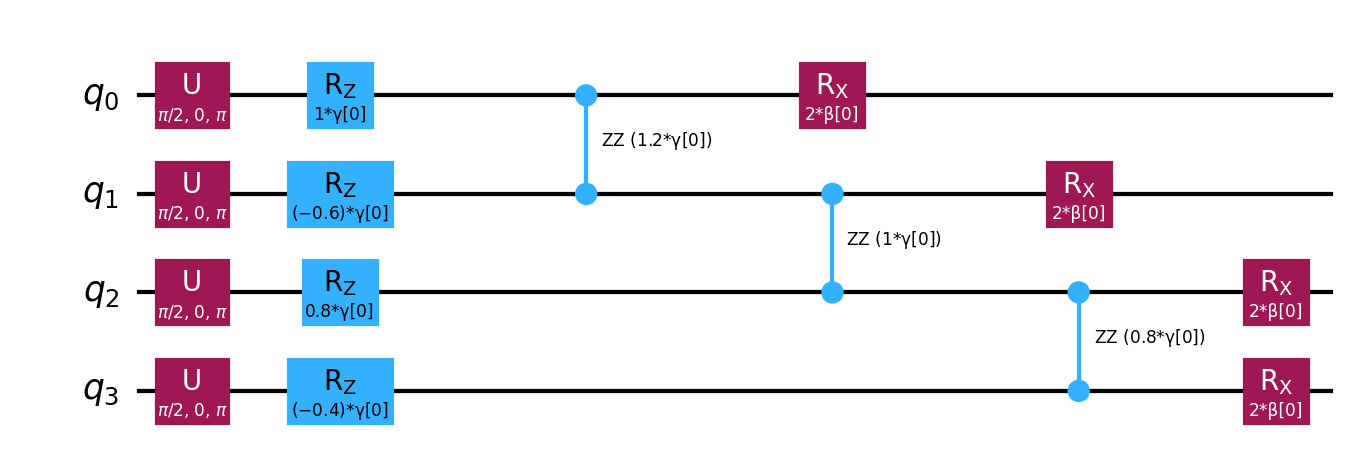
\includegraphics[width=.9\linewidth]{img/qaoa_circuit_fibonacci.png}\\
    {\small Fibonacci, 4 candidates: tridiagonal $Q$ $\Rightarrow$ a chain of $R_{ZZ}$ gates}
\end{frame}

% ===== 5. FIXED ANGLES =====
\begin{frame}{Fixed angles, found once offline}
    \centering
    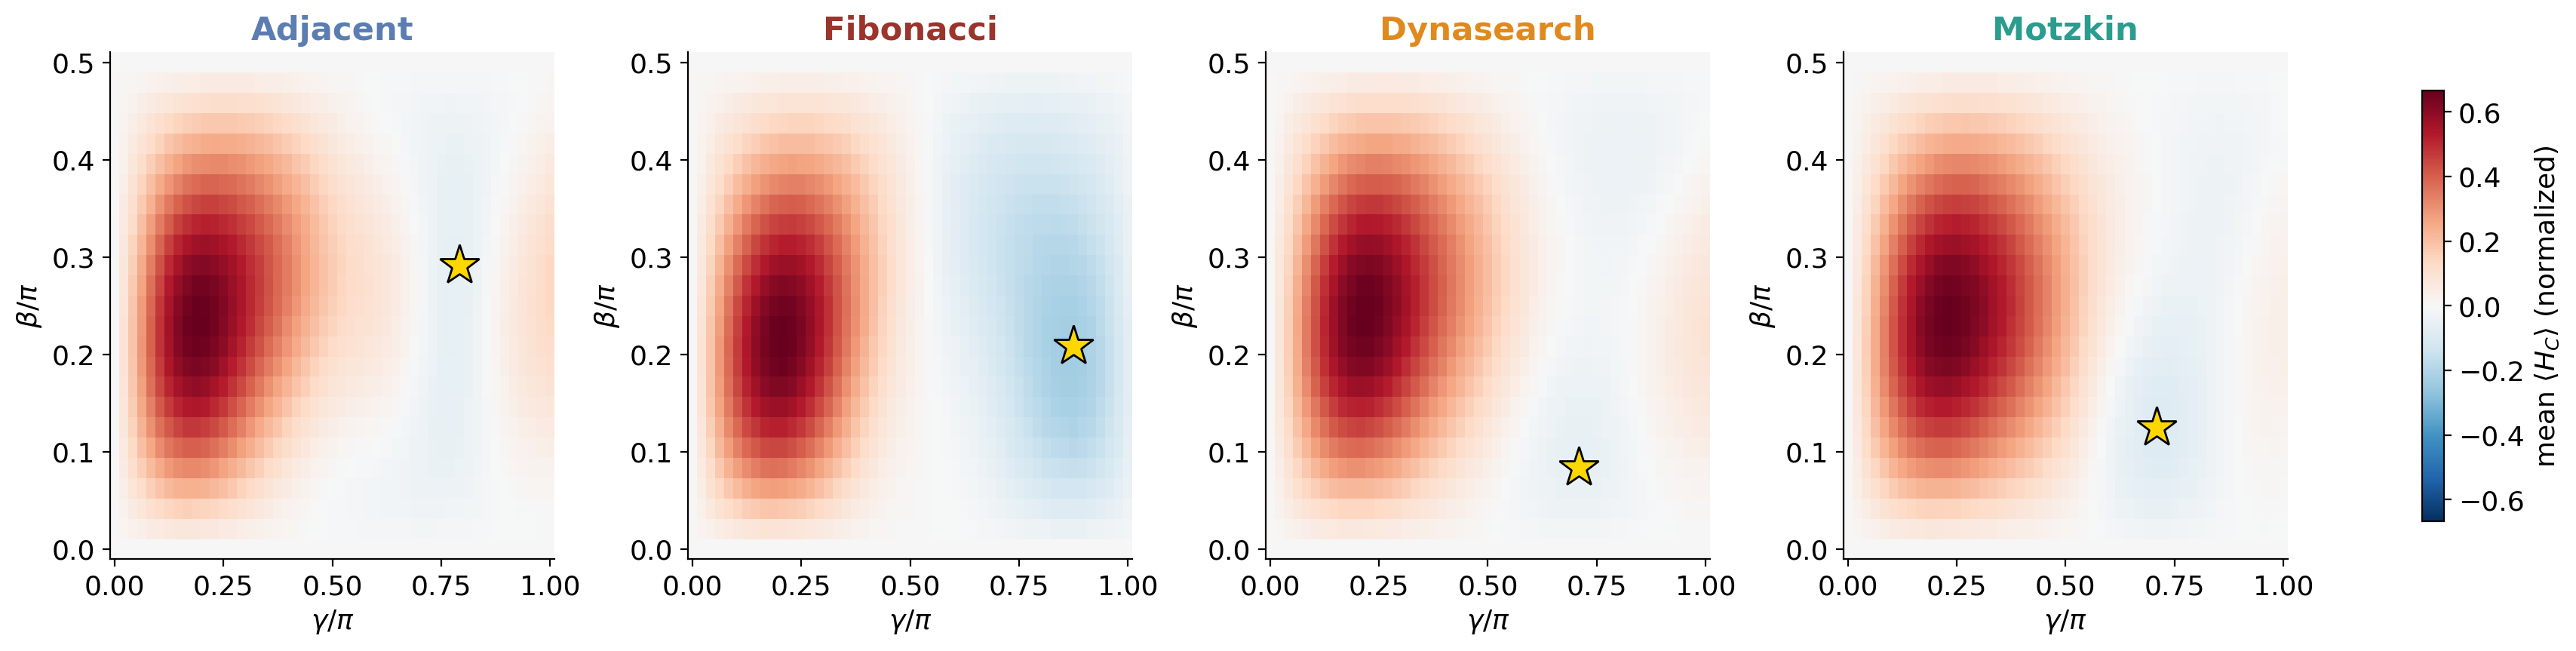
\includegraphics[width=\linewidth,height=.62\textheight,keepaspectratio]{img/landscape.png}\\[1mm]
    {\small mean $\langle H_C\rangle$ over the training windows (statevector), $\star$ = frozen $(\gamma^\star,\beta^\star)$}
    \takeaway{On hardware: \textbf{one submission per move}, no variational loop.}
\end{frame}

% ===== 6. SAMPLE TO MOVE =====
\begin{frame}{From samples to a move}
    \centering
    \begin{tikzpicture}[scale=.82,transform shape,
        st/.style={draw,rounded corners,fill=pwrtwo,align=center,minimum height=1.5cm,text width=2.5cm,thick},
        >={Stealth[length=3mm]}]
        \node[st] (w) at (0,0) {cut $\pi$ into\\windows of 6\\\small(dense nb.)};
        \node[st] (s) at (3.4,0) {4096 shots\\per circuit};
        \node[st] (e) at (6.8,0) {keep the\\\textbf{lowest-energy}\\bitstring};
        \node[st] (r) at (10.2,0) {greedy repair\\across windows};
        \node[st,fill=pwrone,text=white] (m) at (13.6,0) {apply all\\kept swaps};
        \foreach \a/\b in {w/s,s/e,e/r,r/m} \draw[->,thick] (\a) -- (\b);
        \node[below=3mm of e,align=center,font=\small,text=pwrone] {not the most frequent one:\\at $p=1$ it is usually all-zeros};
    \end{tikzpicture}
\end{frame}

% ===== 7. COUPLING MAPS =====
\section{Compilation}
\begin{frame}{Four coupling maps, same four QUBOs}
    \centering
    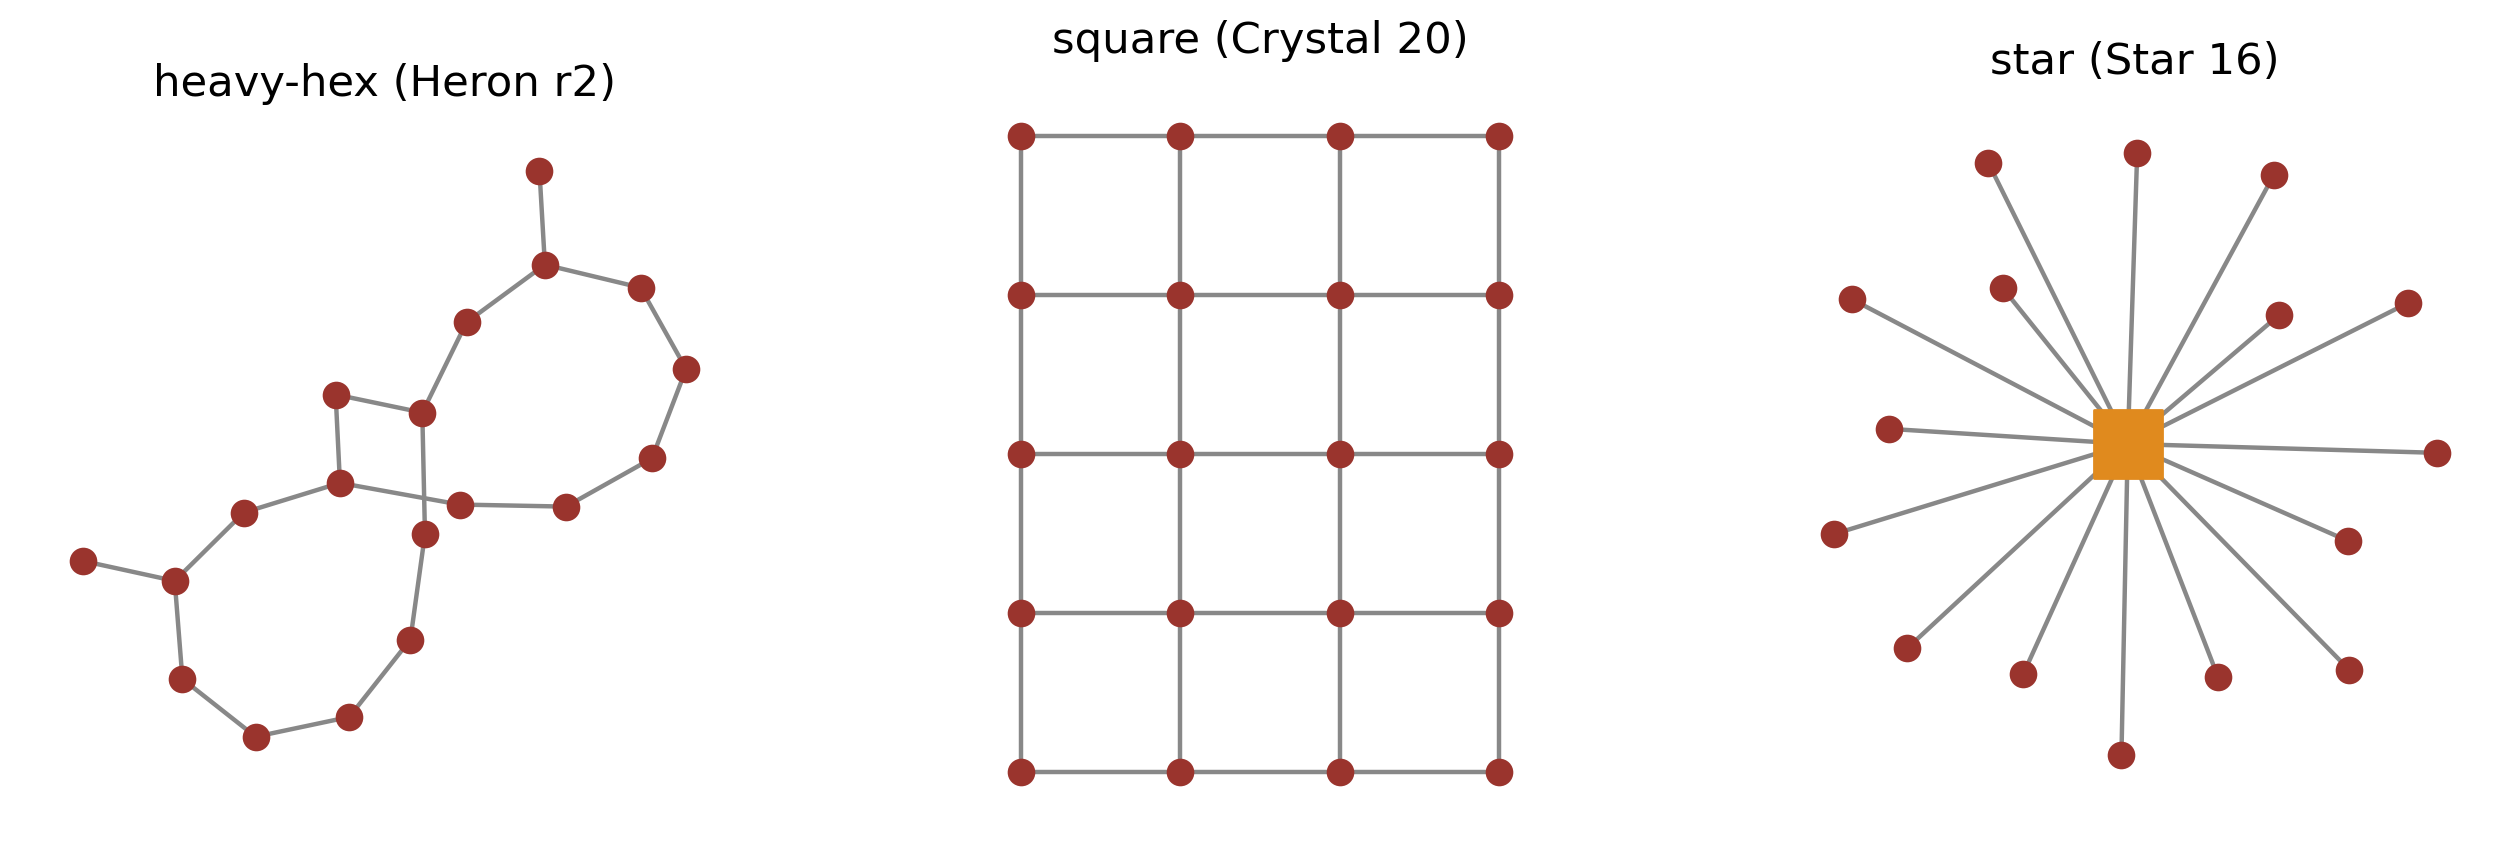
\includegraphics[width=\linewidth,height=.62\textheight,keepaspectratio]{img/coupling_maps.png}\\
    {\small Heron r2 (156 q) \quad Crystal 20 and Crystal 54 \quad Star 16 with a central resonator (MOVE instead of SWAP)}
\end{frame}

% ===== 8. DEPTH =====
\begin{frame}{Compiled depth: the ordering does not depend on the hardware}
    \centering
    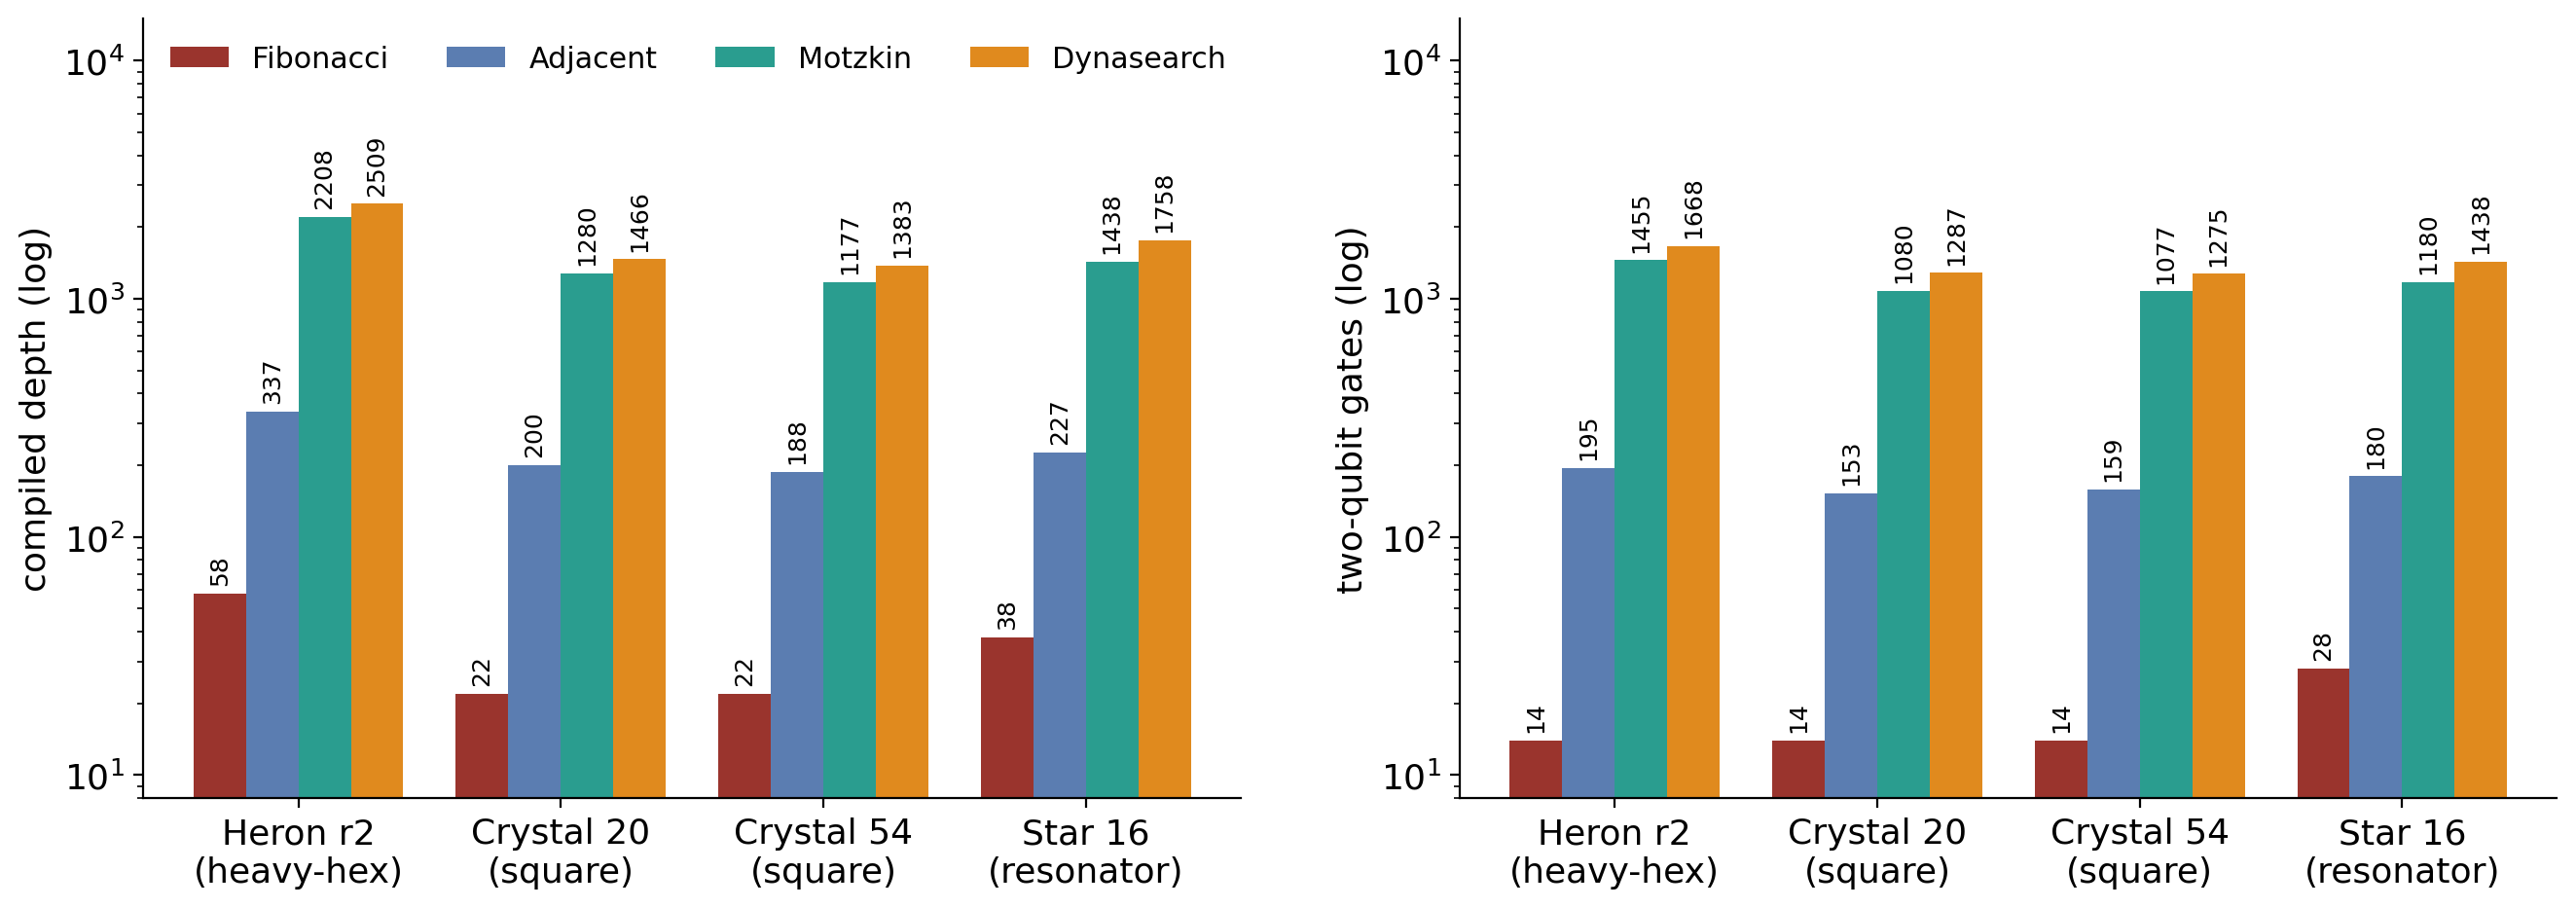
\includegraphics[width=\linewidth,height=.62\textheight,keepaspectratio]{img/depth.png}
    \takeaway{Fibonacci $\ll$ Adjacent $\ll$ Motzkin $<$ Dynasearch on every map --- the same order as on the annealer.}
\end{frame}

% ===== 9. HW PRD =====
\section{Hardware}
\begin{frame}{IBM Heron r2: one QAOA move, 10 Taillard $20\times5$ instances}
    \centering
    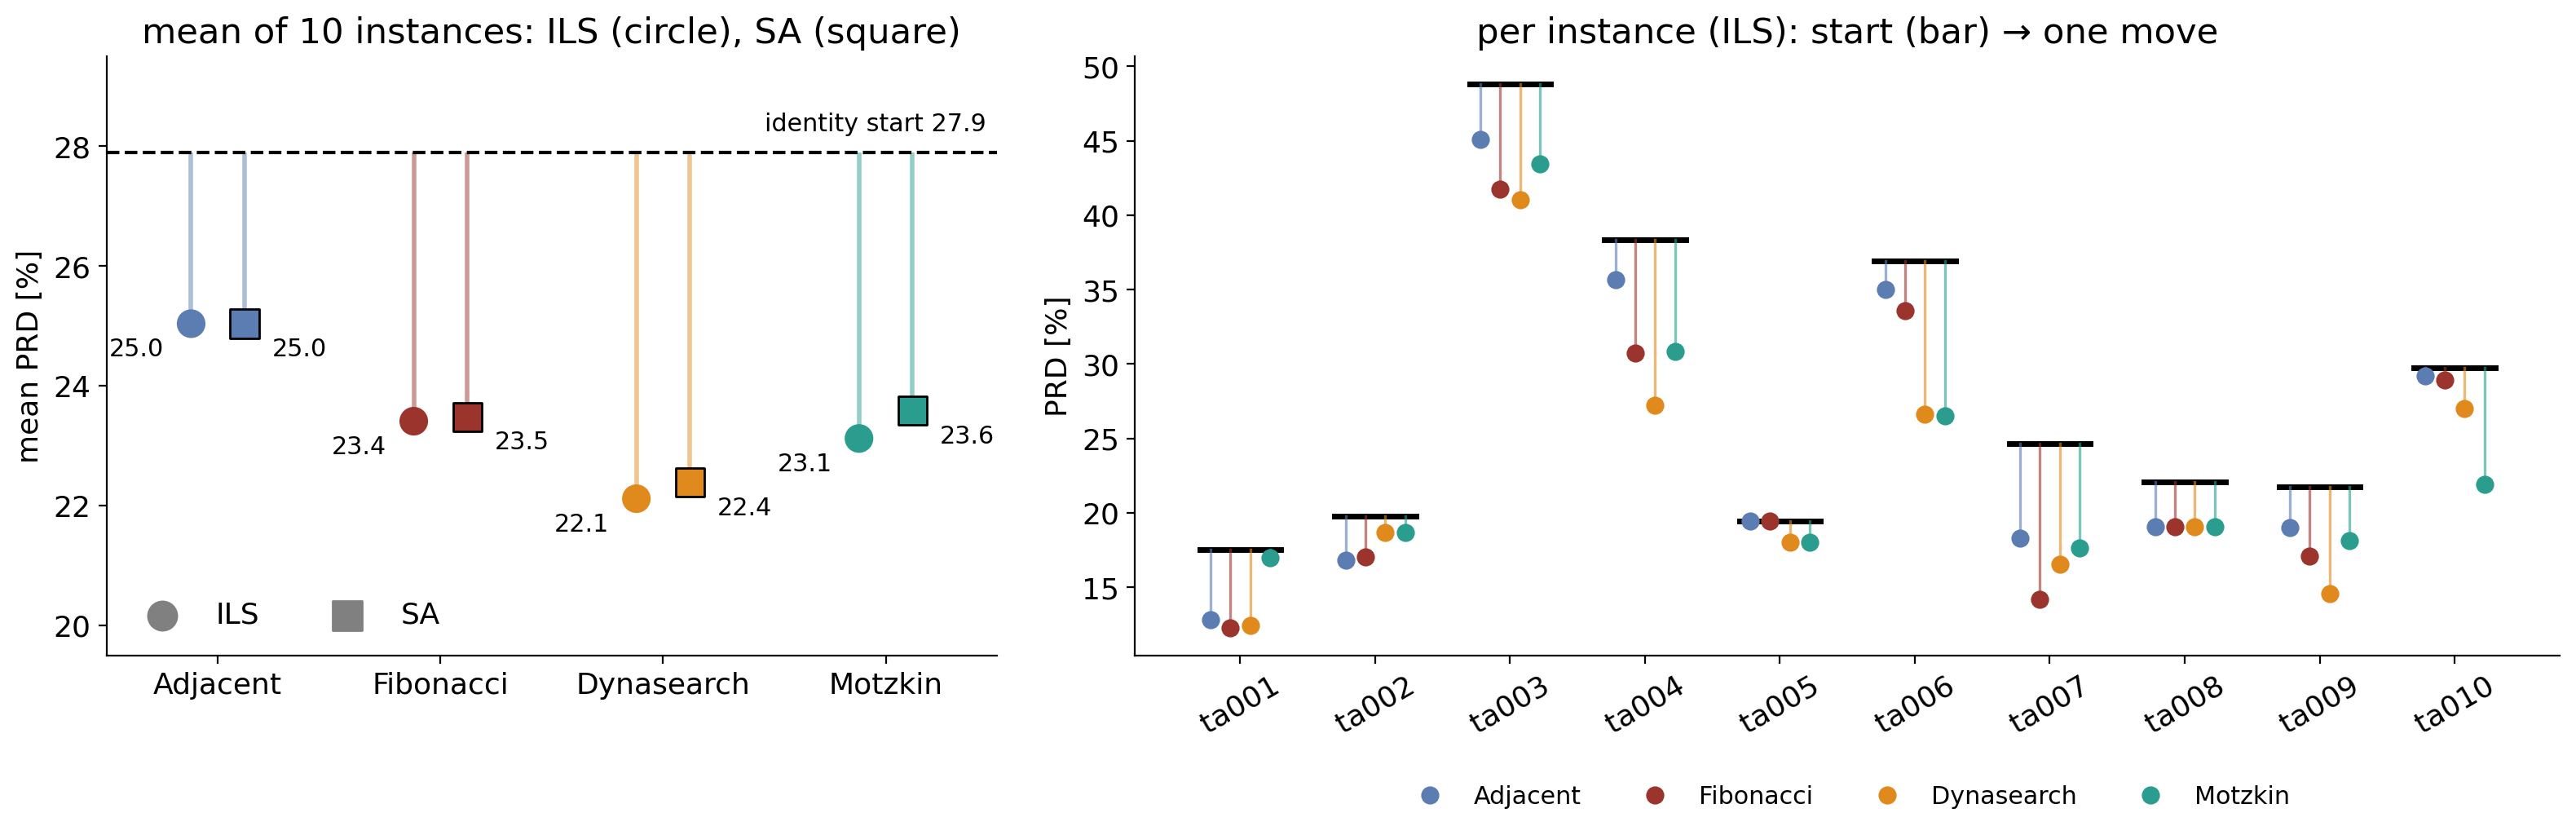
\includegraphics[width=\linewidth,height=.62\textheight,keepaspectratio]{img/hw_prd.png}
    \takeaway{80 runs, $\approx$460 s QPU. One move: PRD $27.9 \to 22.1$--$25.0$.}
\end{frame}

% ===== 10. TIME =====
\begin{frame}{Why only one move: queue, not computation}
    \centering
    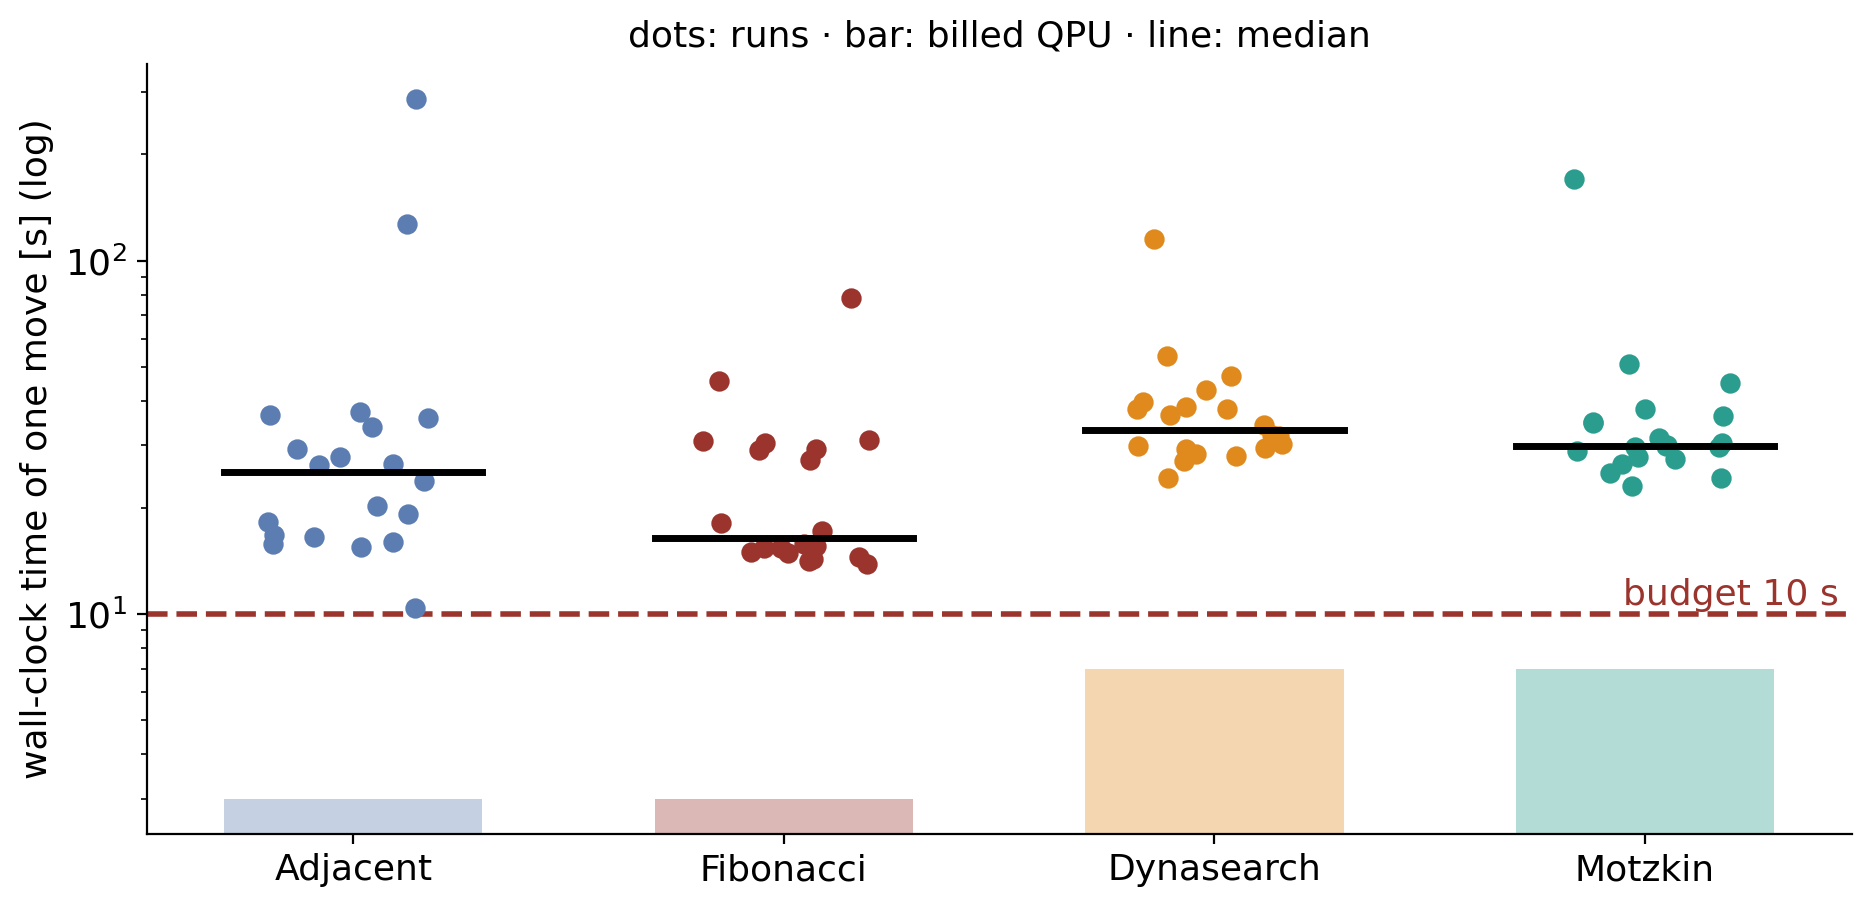
\includegraphics[width=.82\linewidth,height=.62\textheight,keepaspectratio]{img/hw_time.png}
    \takeaway{3--7 s of QPU, 10--288 s on the clock $\Rightarrow$ no run reached a second move.}
\end{frame}

% ===== 11. COMPARE =====
\begin{frame}{Gate model vs.\ annealer vs.\ classical}
    \centering
    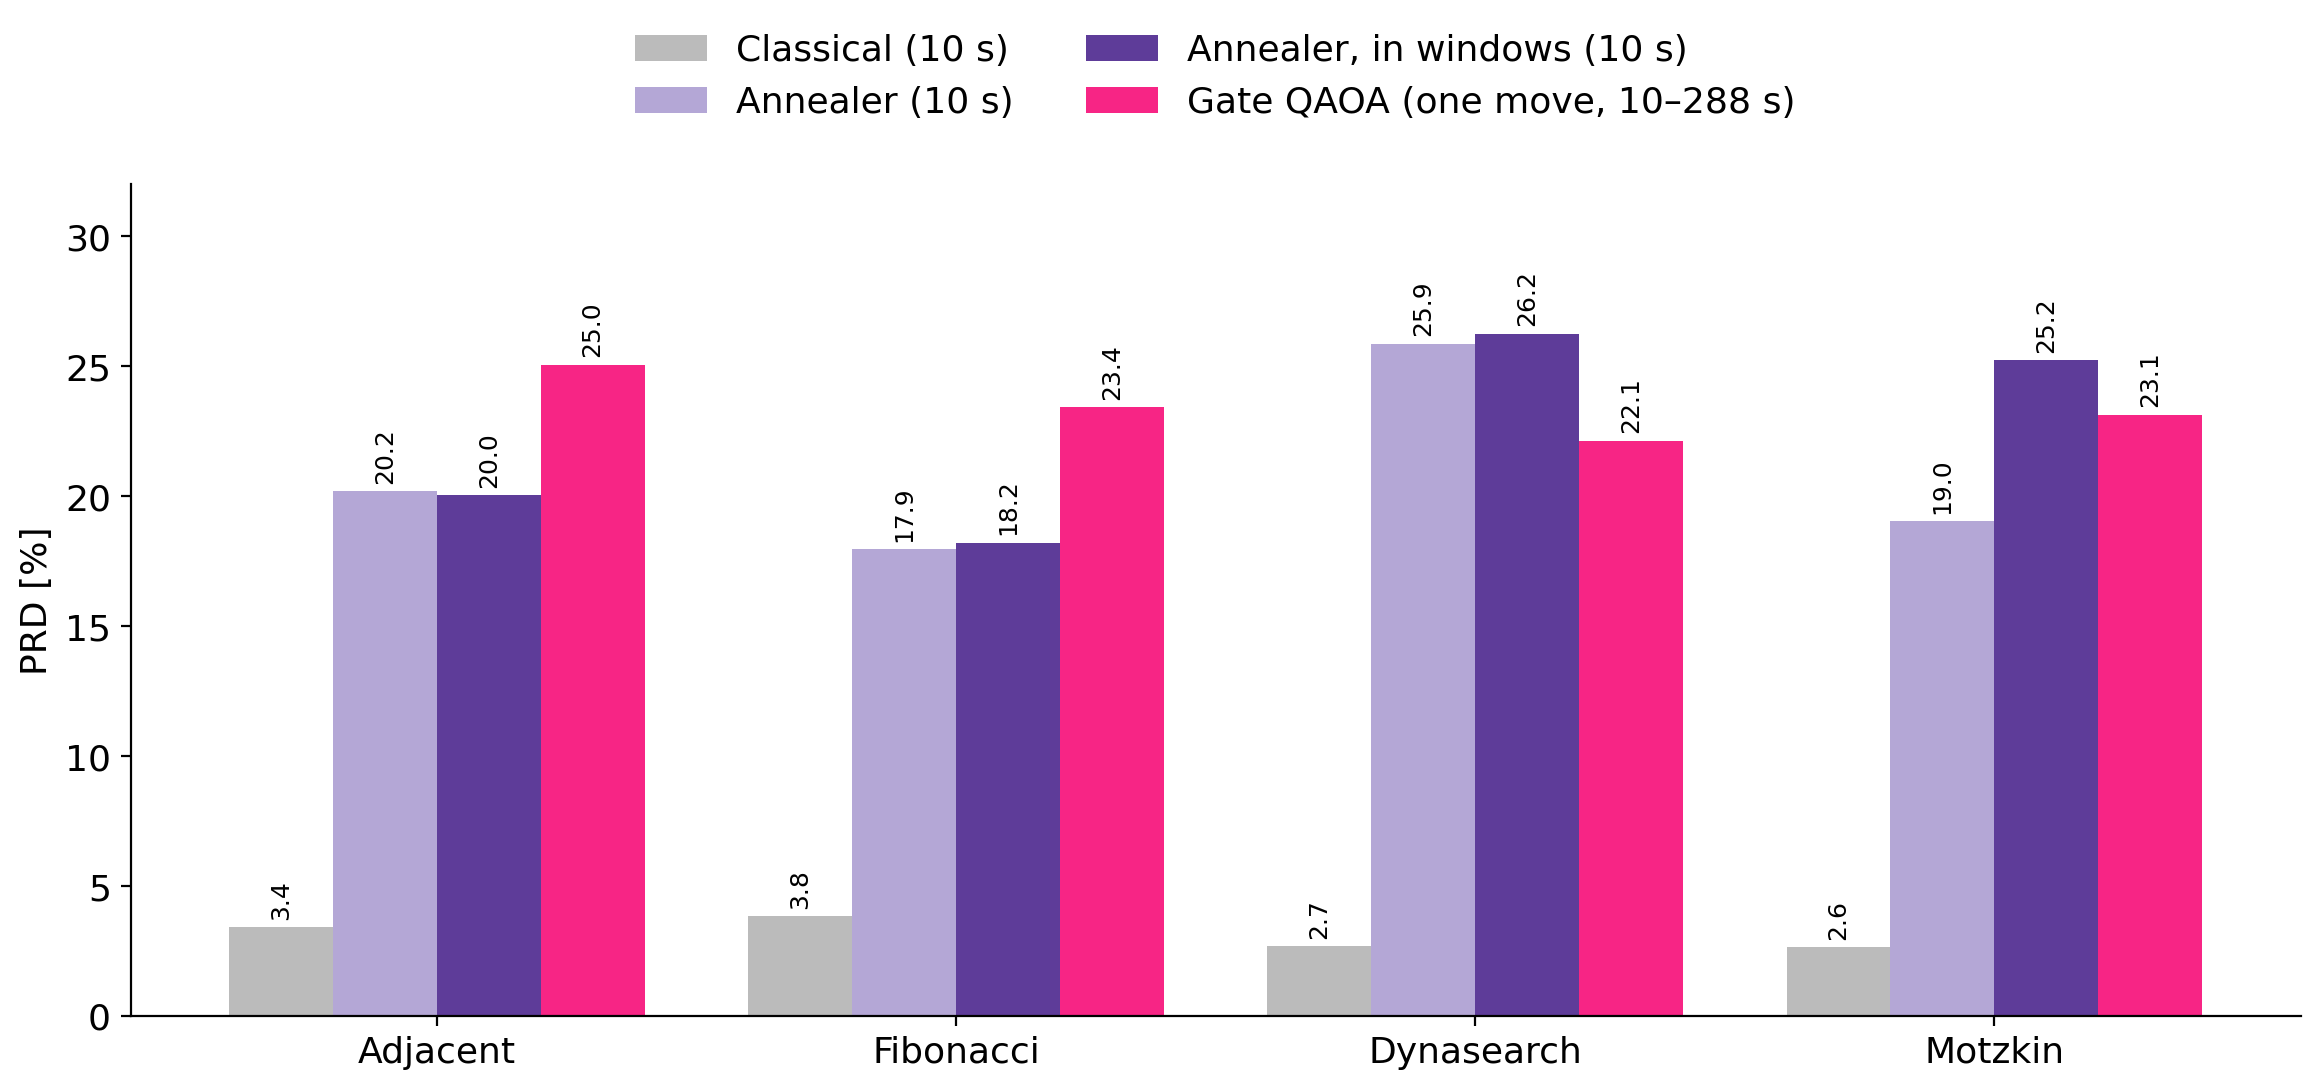
\includegraphics[width=.92\linewidth,height=.62\textheight,keepaspectratio]{img/compare.png}
    \takeaway{Gate QAOA wins on Dynasearch; all quantum back-ends stay far behind classical evaluation.}
\end{frame}

% ===== 12. THREE MAPS =====
\begin{frame}{Same circuits on three processors}
    \centering
    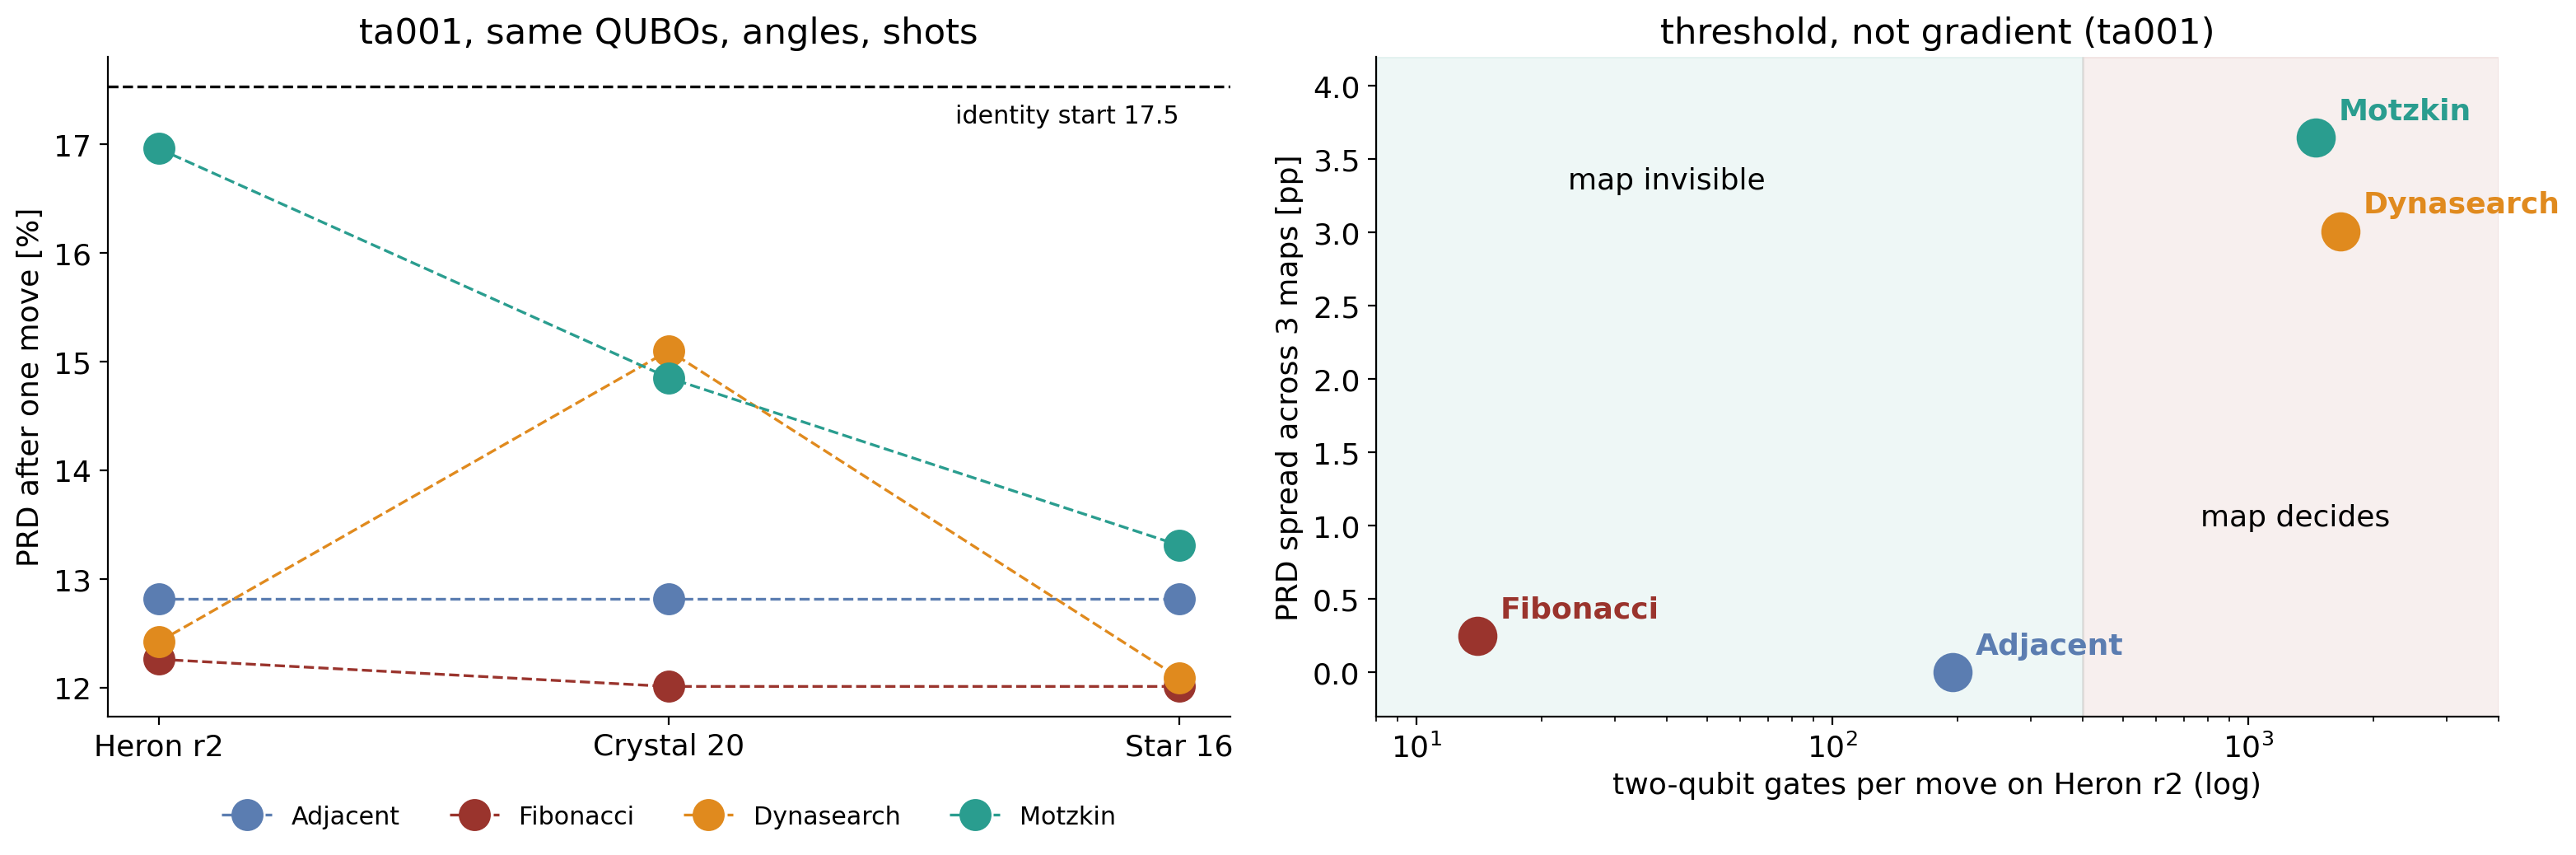
\includegraphics[width=\linewidth,height=.62\textheight,keepaspectratio]{img/arch.png}
    \takeaway{Short circuits: identical $C_{\max}$ on 156 and 16 qubits. Deep circuits: the map decides.}
\end{frame}

% ===== 13. CONCLUSIONS =====
\section{Conclusions}
\begin{frame}{Take-home}
    \begin{columns}[T]
        \begin{column}{.32\textwidth}
            \centering
            {\Huge\color{pwrone} 1}\\[1mm]
            \textbf{Depth = embedding}\\
            \small compiled depth plays the role of annealer embedding capacity
        \end{column}
        \begin{column}{.32\textwidth}
            \centering
            {\Huge\color{pwrone} 2}\\[1mm]
            \textbf{Threshold}\\
            \small below it the coupling map is invisible, above it the map decides
        \end{column}
        \begin{column}{.32\textwidth}
            \centering
            {\Huge\color{pwrone} 3}\\[1mm]
            \textbf{Cost per move}\\
            \small one submission, $\approx$30 s wall-clock; billing grows with the number of circuits
        \end{column}
    \end{columns}
    \vspace{8mm}

    \centering\small
    Next: full protocol (10 instances $\times$ 5 seeds $\times$ 6 budgets) on every map, larger $n$.\\[3mm]
    Code, angles and data: \texttt{doi.org/10.5281/zenodo.24106982}
\end{frame}

% ===== 14. THANKS =====
\begin{frame}
    \centering\vfill
    {\Huge\color{pwrone} Thank you}\\[6mm]
    {\large Questions?}\\[8mm]
    
\includegraphics[height=12mm]{logo_PWR.png}
    \vfill
\end{frame}

\end{document}
